\section{Experimental Results and Discussion}

%%%% BECHMARKS
\begin{table*}[t]
\begin{center}
\begin{small}
\begin{tabular}{llll}
\hline
\textbf{Task} & \textbf{Benchmark} & \textbf{\textit{in-domain} Test set} & \textbf{\textit{out-of-domain} Test set} \\ \hline
POS-Tagging & (Acc.) 0.972 \cite{Toutanova:2003} & 0.959 (skip-gram negsam+up) & 0.910 (skip-gram negsam+noup)\\ 
Chunking & (F1) 0.942 \cite{Sha:2003} & 0.938 (Brown cluster v2000) & 0.676 (glove+noup)\\  
NER & (F1) 0.893 \cite{Ando:2005} & 0.868 (skip-gram negsam+noup) & 0.736 (skip-gram negsam+noup) \\  
MWE & (F1) 0.625 \cite{Schneider+:2014} & 0.654 (cw+up) & - \\ 
\hline
\end{tabular}
\caption{Benchmark results vs. our best results for in-domain and out-of-domain test sets (Acc. refers to Accuracy; F1 refers to F1-measure).}
\label{benchmark}
\end{small}
\end{center}
\end{table*}

%%%%%%%%%%%%%%%%%%%%%%%%%%%%
%%% HEATMAPS 
\begin{figure*}
\centering
\begin{subfigure}{7cm}
	\centering
    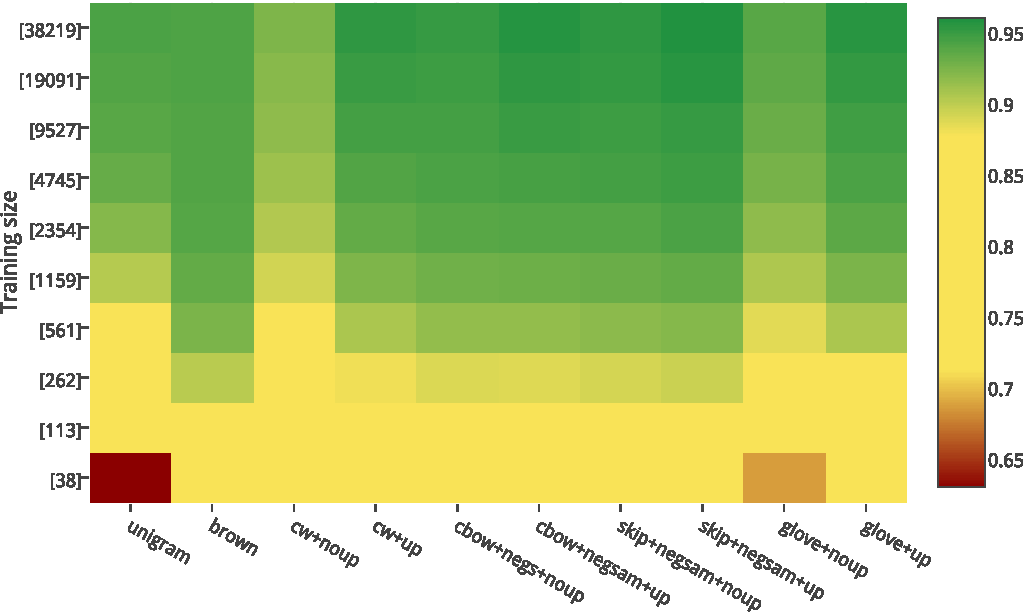
\includegraphics[scale=0.4]{plots/map-pos-color-invert}    	
	\subcaption{POS-Tagging Accuracy}	
	\label{pos}
\end{subfigure}
\begin{subfigure}{7cm}
	\centering
    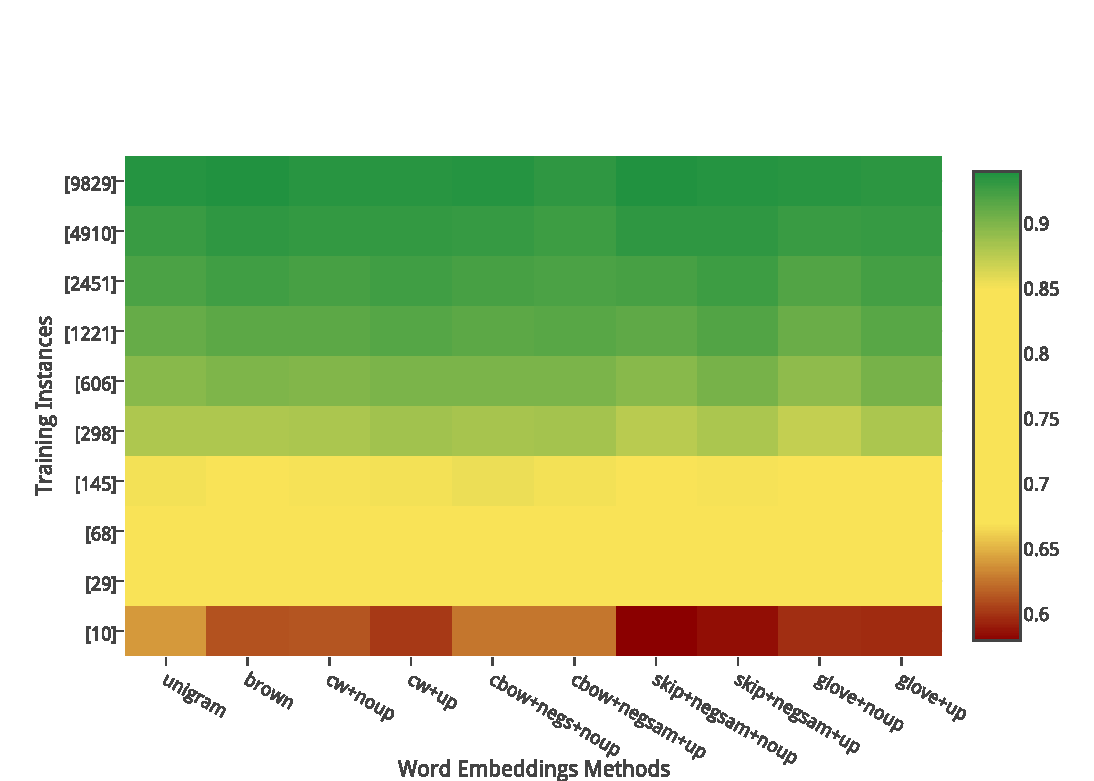
\includegraphics[scale=0.4]{plots/map-chunk-color-invert}
	\subcaption{Chunking F1-Measure}	
	\label{chu}
\end{subfigure}
%\\[-1.5ex]  %%<-- in this line
\begin{subfigure}{7cm}
	\centering
    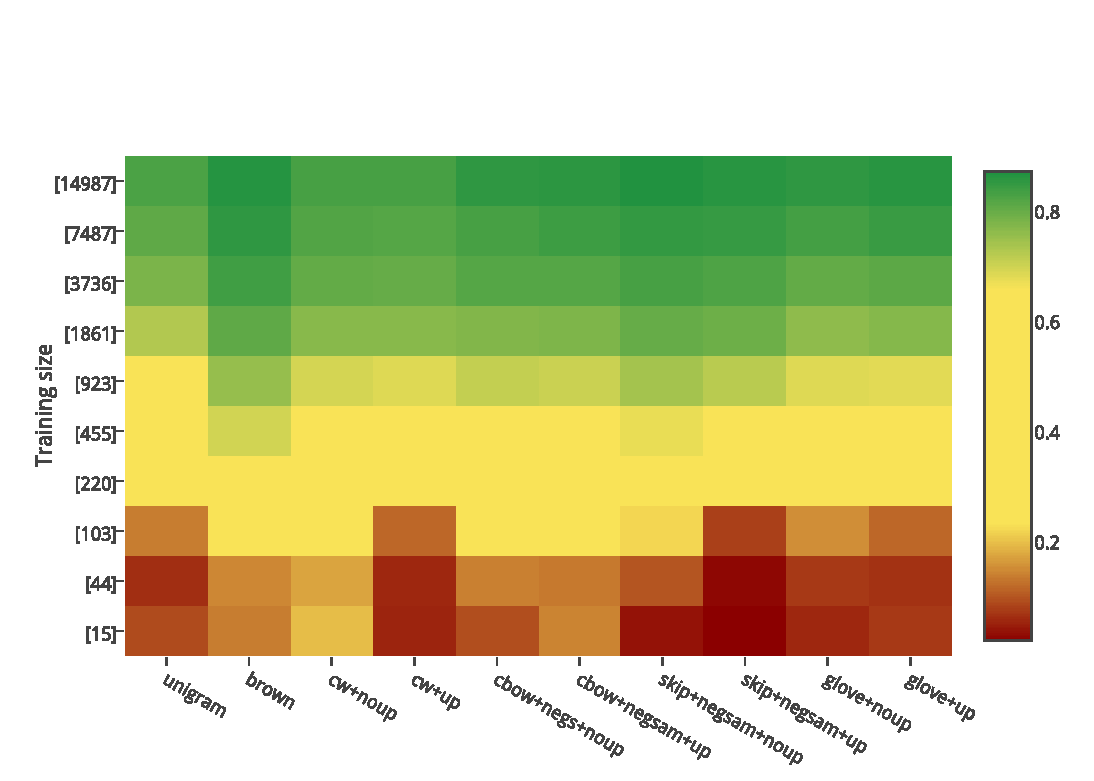
\includegraphics[scale=0.4]{plots/map-ner-color-invert}    	
	\subcaption{NER F1-Measure}	
	\label{ner}
\end{subfigure}
\begin{subfigure}{7cm}
	\centering
    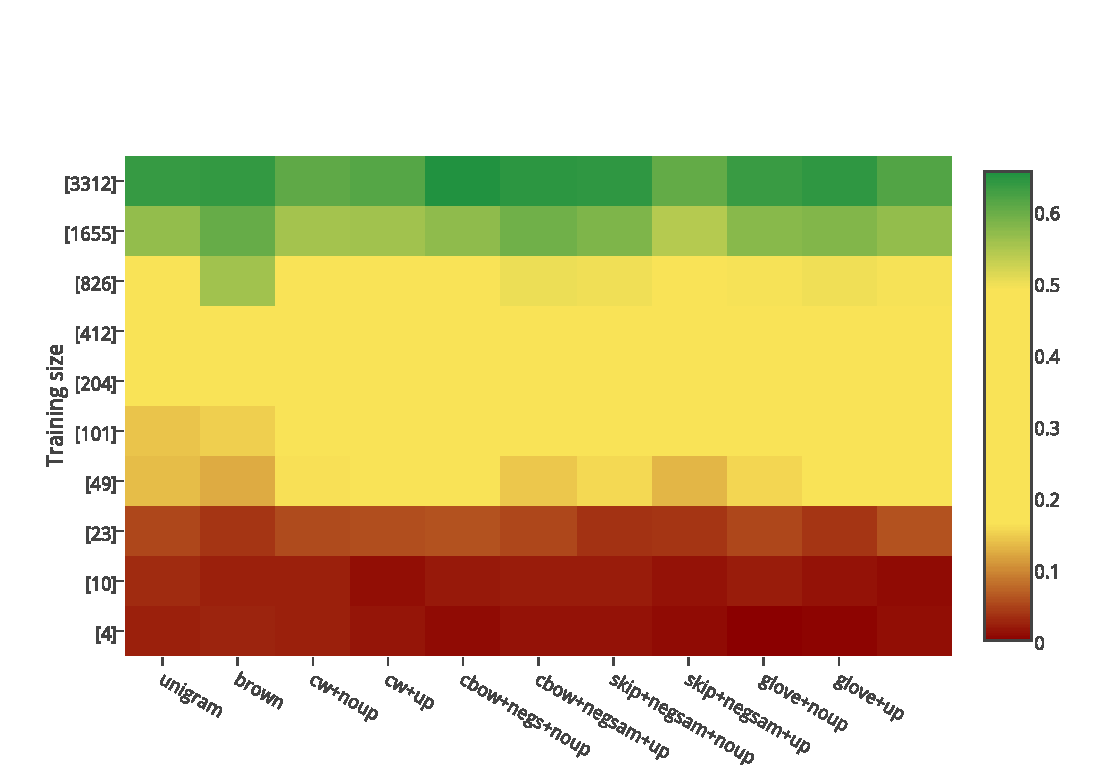
\includegraphics[scale=0.4]{plots/map-mwe-color-invert}
	\subcaption{MWEs F1-Measure}		
	\label{mwe}
\end{subfigure}
\caption{Best results for each method for POS-Tagging, Chunking, NER and MWE identification. The x-axis correspond to the different word embeddings methods and the y-axis to the 10 training partitions at log scale. Green color stand for high performance, while red color stands for low performance. The methods are in chronological order; wherein the suffix \textit{up} stands for \textit{updated or fine-tuned features}, and \textit{noup} stands for \textit{no-updated} features.\nss{[The rightmost axis labels of (c) are cut off. Also, is it possible to enlarge the axis text at all? Difficult to read when printed.]}}
\label{fig:heatmaps}
\end{figure*}


%%%%%%%%%%%%%%%%%%%%%%%%%%%%
%%% Vector fields
% POS
\begin{figure*}
\centering
\begin{subfigure}[b]{0.48\textwidth}
	\centering
    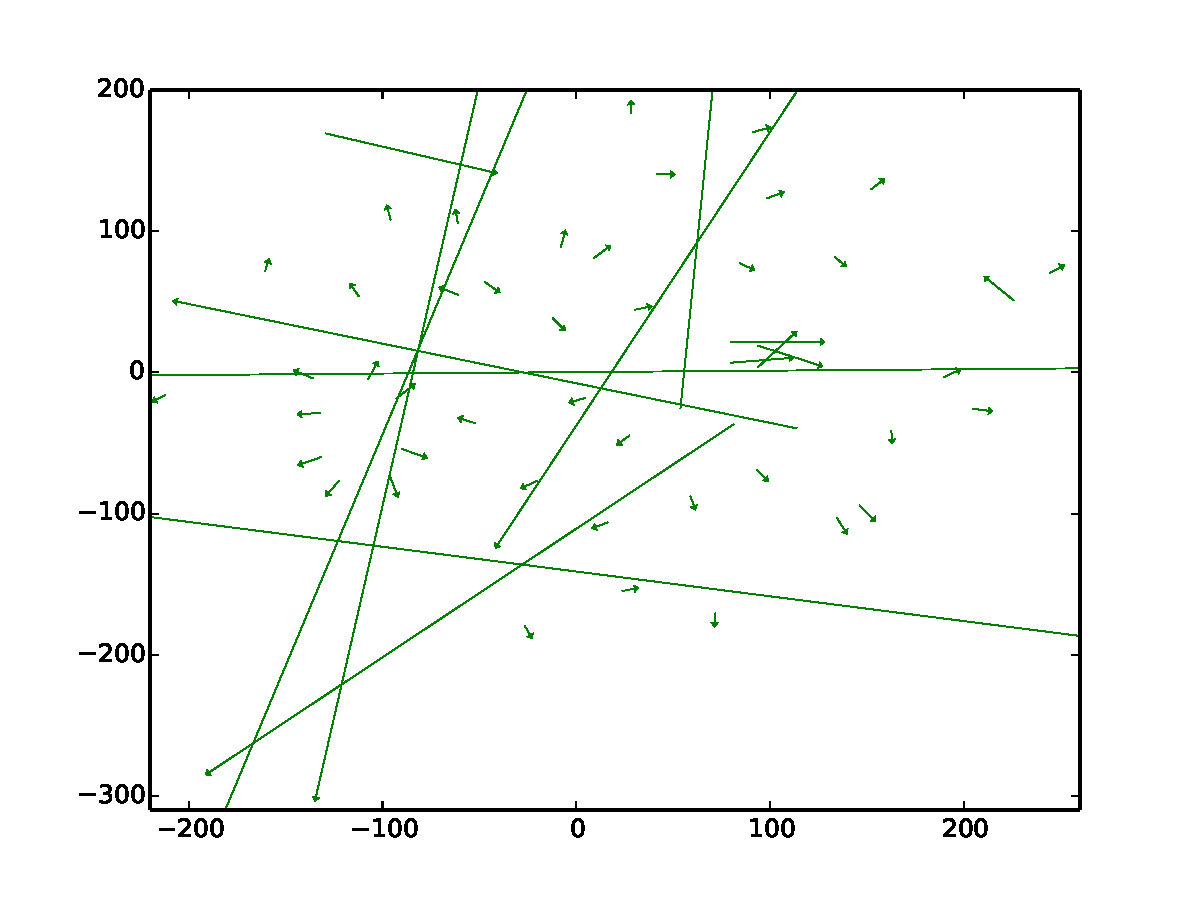
\includegraphics[width=\textwidth]{plots/vectorField/Lizhen/scaled/Lizhen_skip_chunking}
	\subcaption{Chunking}	
	\label{fig:skipChu}
\end{subfigure}
\begin{subfigure}[b]{0.48\textwidth}
	\centering
    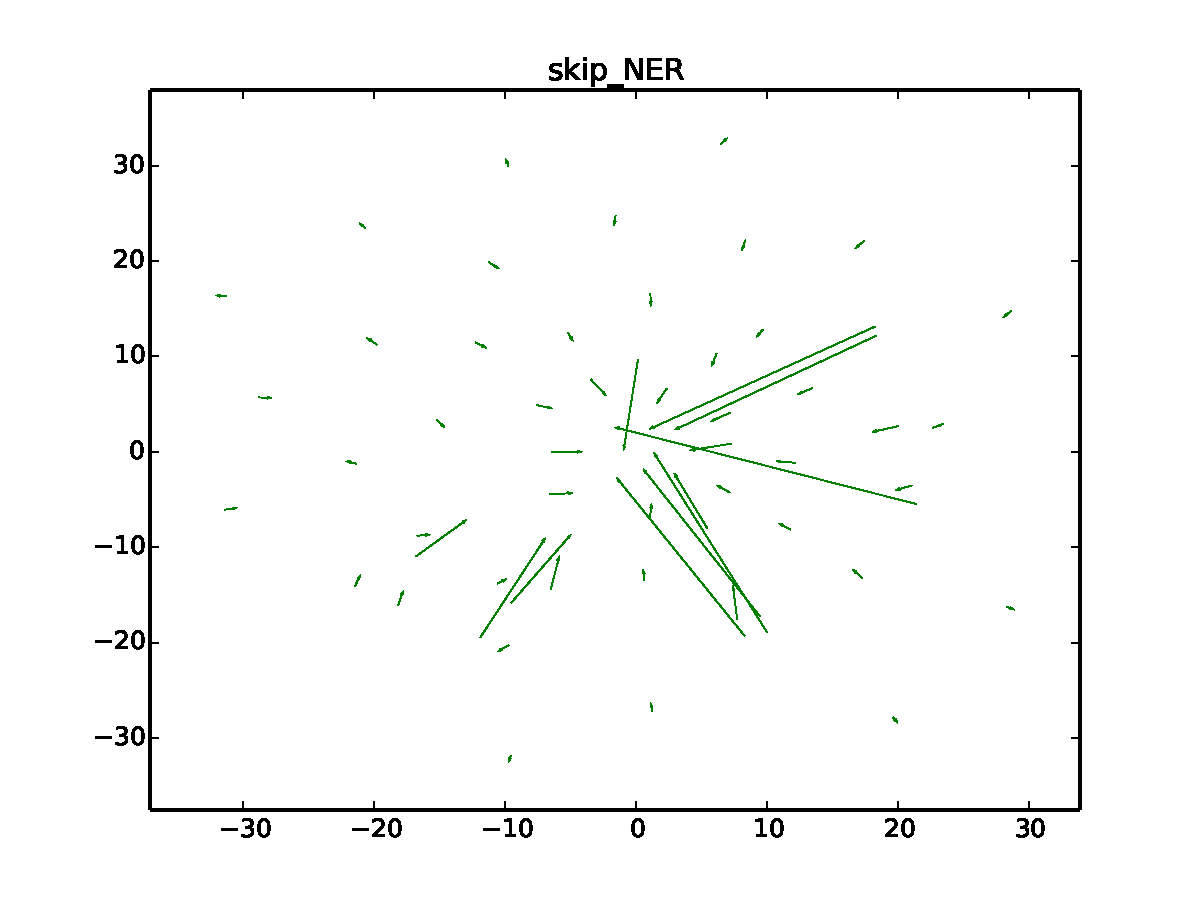
\includegraphics[width=\textwidth]{plots/vectorField/Lizhen/Lizhen_skip_NER}    	
	\subcaption{NER}
	\label{fig:skippos}	
\end{subfigure}
%\begin{subfigure}[b]{0.48\textwidth}
%	\centering
%   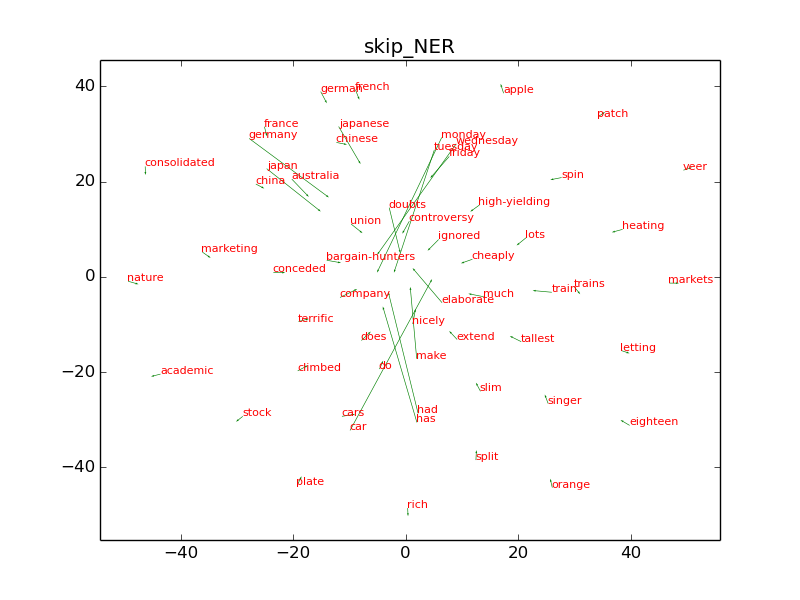
\includegraphics[width=\textwidth]{plots/vectorField/skip_NER.png}
%	\label{fig:skipner}
%	\subcaption{}	
%\end{subfigure}
%%\begin{subfigure}{6cm}
%	\centering
 %   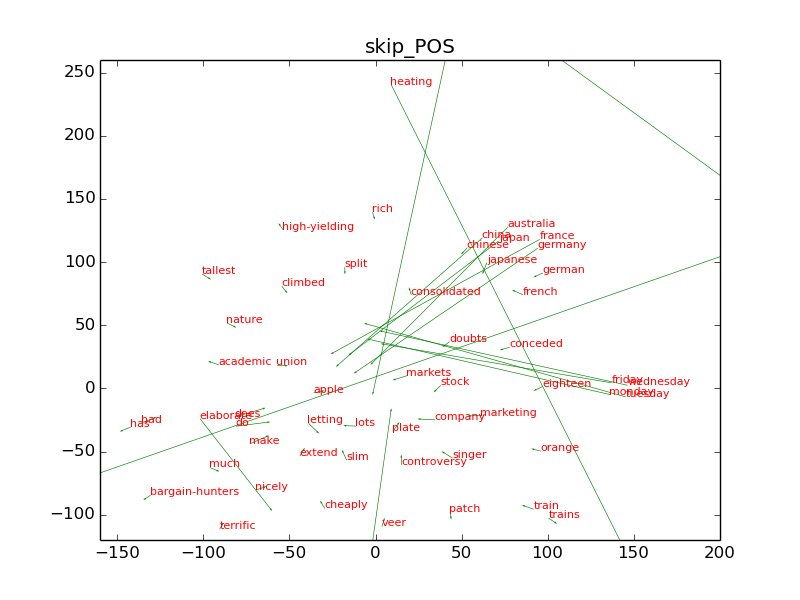
\includegraphics[scale=0.3]{plots/vectorField/skip_POS.png}
%	\label{fig:skipmwe}
%	\subcaption{}	
%\end{subfigure}
\caption{Updated vs.\ no-updated word representations for POS-tagging and chunking using skip-gram\nss{[Arrowheads are too small to see]}}
\label{fig:vectorfield}
\end{figure*}

We focus on the following questions:

%\textbf{(i) Are the evaluated word embedding methods better than unigram features?}
\textbf{(i) Are some word embeddings better than the baseline approaches of one-hot unigram features and Brown clusters?}
To answer this question we systematically compared the usefulness of word embedding versus
unigram and Brown cluster features for sequence tagging.
As shown in \tabref{benchmark}, every task has at least one word embedding method that outperforms
unigram features. In the case of chunking, Brown clustering performs slightly better than other methods \nss{on in-domain data} when the model is trained with all training data. 


%\textbf{(ii) How does the size of labelled training data affect the experimental results?}
\textbf{(ii) Do word embedding features help more than unigram features to achieve decent performance with limited labelled training data?}

\figref{fig:heatmaps} shows that for POS-tagging and NER, with only several hundred training instances, 
word embedding features are especially helpful relative to unigram features. 
For example, when trained with 561 instances, the POS-tagging model using skip-gram embeddings with fine-tuning is 5.3\% above
the one with unigram features; and when trained with 932 instances, the NER model using skip-gram embeddings without fine-tuning is 11.7\% above the one using unigrams. 
Similar improvements are also found for other types of word embeddings and Brown clustering, when the training set is small. 
However, all kinds of word representations perform similarly in chunking regardless of the size of training set. 
For MWE identification, Brown clustering performs slightly better than other methods when trained with approximately 25\% of training instances. Therefore, we conjecture that the POS and NER tasks benefit more from distributional similarity than chunking and MWE identification.

\textbf{(iii) Is fine-tuning helpful for all kinds of word embeddings and across all tasks?}
We found that fine-tuning can correct poorly learned word representations, but can harm well pre-trained ones due to overfitting. For example, CW and Glove perform significantly worse than skip-gram in both POS and NER without fine-tuning, but \emph{with} fine-tuning, the gap between their results and the best performing method becomes smaller. In contrast, skip-gram performs worse on the test set when fine-tuning is applied, though the results on the validation set shows that skip-gram with fine-tuning performs 1\% better, which is a clear sign of overfitting.
%Across all the methods, fine-tuning is helping POS-Tagging and MWE, where the CW method has been found to be the most sensible to tuning, reaching almost 3 points more, when tuning is performed (Figure \ref{pos}, \ref{mwe}).  For chunking and NER, the best results are fine-tuned, but the difference across all the methods and updated features versus not-updated ones, is not significant (Figure \ref{chu}, \ref{ner}). 

To illustrate the effect of fine-tuning, we sampled 60 words and plotted the changes of their word embeddings before and after fine-tuning, by using vector fields. Each arrow points to the direction of change and the size of the arrow indicates the magnitude of change.  Half of the words were chosen manually and include some known word clusters like names of the days and names of countries so that we can observe the changes of word clusters.  The rest of the words were randomly selected (additional plots with 100 randomly sampled words and the top 100 most frequent words, for all the methods and all the tasks, can be found in the supplementary material and at \url{https://123abc123abd.wordpress.com/}).

In \figref{fig:vectorfield}, we show vector fields plots for chunking and NER using skip-gram embeddings.
As illustrated in \figref{fig:skipChu}, after fine-tuning for chunking, all the vectors are changed with similar magnitude 
(except for a few outliers), but their directions of change appear to be random, 
whether they previously belonged to the same word cluster or not.\nss{[I don't understand how clusters are shown in the plots.]} 
In contrast, after fine-tuning for NER, word vectors belonging to the same cluster changed their magnitude and direction homogeneously (\figref{fig:skippos}).\nss{[Why is this good?]} 
The different ways of changing word clusters between the two tasks is another piece of evidence that information contained in word embeddings is less beneficial for chunking than for NER. 


% This also indicates that the graph transformer can identify useful factors in word representations and keep them during training.
\textbf{(iii) How well do the word embeddings perform when evaluated on \textit{out-of-domain} test sets?}
\tabref{benchmark} shows \textit{out-of-domain} performance on all the tasks for which out-of-domain data is available.
As expected, the performance drops across the board. The difference is most pronounced for chunking, which loses nearly 30\% absolute for word embedding methods as well as for unigrams, 
indicating that word embeddings and unigram features provide similar information 
for chunking. 


Another interesting observation is that fine-tuning is likely to harm out-of-domain performance because the distribution between in-domain and out-of-domain datasets is different. This suggests that word embeddings pre-trained in an unsupervised way capture more common properties across domains. 

\textbf{(iv) How well do the word embeddings perform for unknown words?}
We also isolate performance on out-of-vocabulary (OOV) words 
in the \textit{in-domain} and \textit{out-of-domain} settings (\figref{OOV}).
As expected, word embeddings and Brown clustering excel in out-of-domain OOV performance.
Word embeddings without\nss{[with?]} fine-tuning are more successful for 
in-domain than out-of-domain datasets, since fine-tuned
word representations become task-specific\nss{[not only task-specific, but domain-specific?]}. 
In addition, OOV performance tends to be insensitive to the size of training sets.



Finally, we address the following question: \textbf{(vi) It has been shown that Brown clusters are useful features for MWE identification; is there any additional benefit to word embeddings for this task?} 
According to our experiments, the word embedding features distilled by fine-tuned CW reached the best results, beating the state-of-the-art performance (see \tabref{benchmark}).
However, the difference between Brown clustering and fine-tuned CW is not impressive, suggesting that distributed word representations and cluster-based representations captures similar features for the MWE identification task. Moreover, we observe that this is the most difficult of the four tasks: it has less training data and achieves the lowest score.


In this paper, we do not aim to maximise the absolute performance of the tasks under 
study, but rather to study the impact of word embeddings for sequence tagging tasks under controlled settings. Thus the performance of our systems in NER, POS and chunking are slightly worse than the best ones in benchmarks (\tabref{benchmark}). The 2.7\% difference between our NER system and the best performing system is due to the fact that we use a first-order instead of a second-order CRF~\cite{Ando:2005}. 
\nss{[In the following sentences, should ``baselines'' be ``benchmarks''?:]}Another difference between our implementation and the baselines is that we tuned the hyperparameters with random search, so that the experiments can be easily replicated by using the same random seed. In contrast, the hyper-parameters of the baselines are tuned by experts, which are difficult to reproduce. For the task of MWE identification, our implementation and settings beat the baseline.




%%%%%%%%%%%%%%%%%%%%%%%%%%%%
%%% OOV 
\begin{figure*}[t]
\centering
    	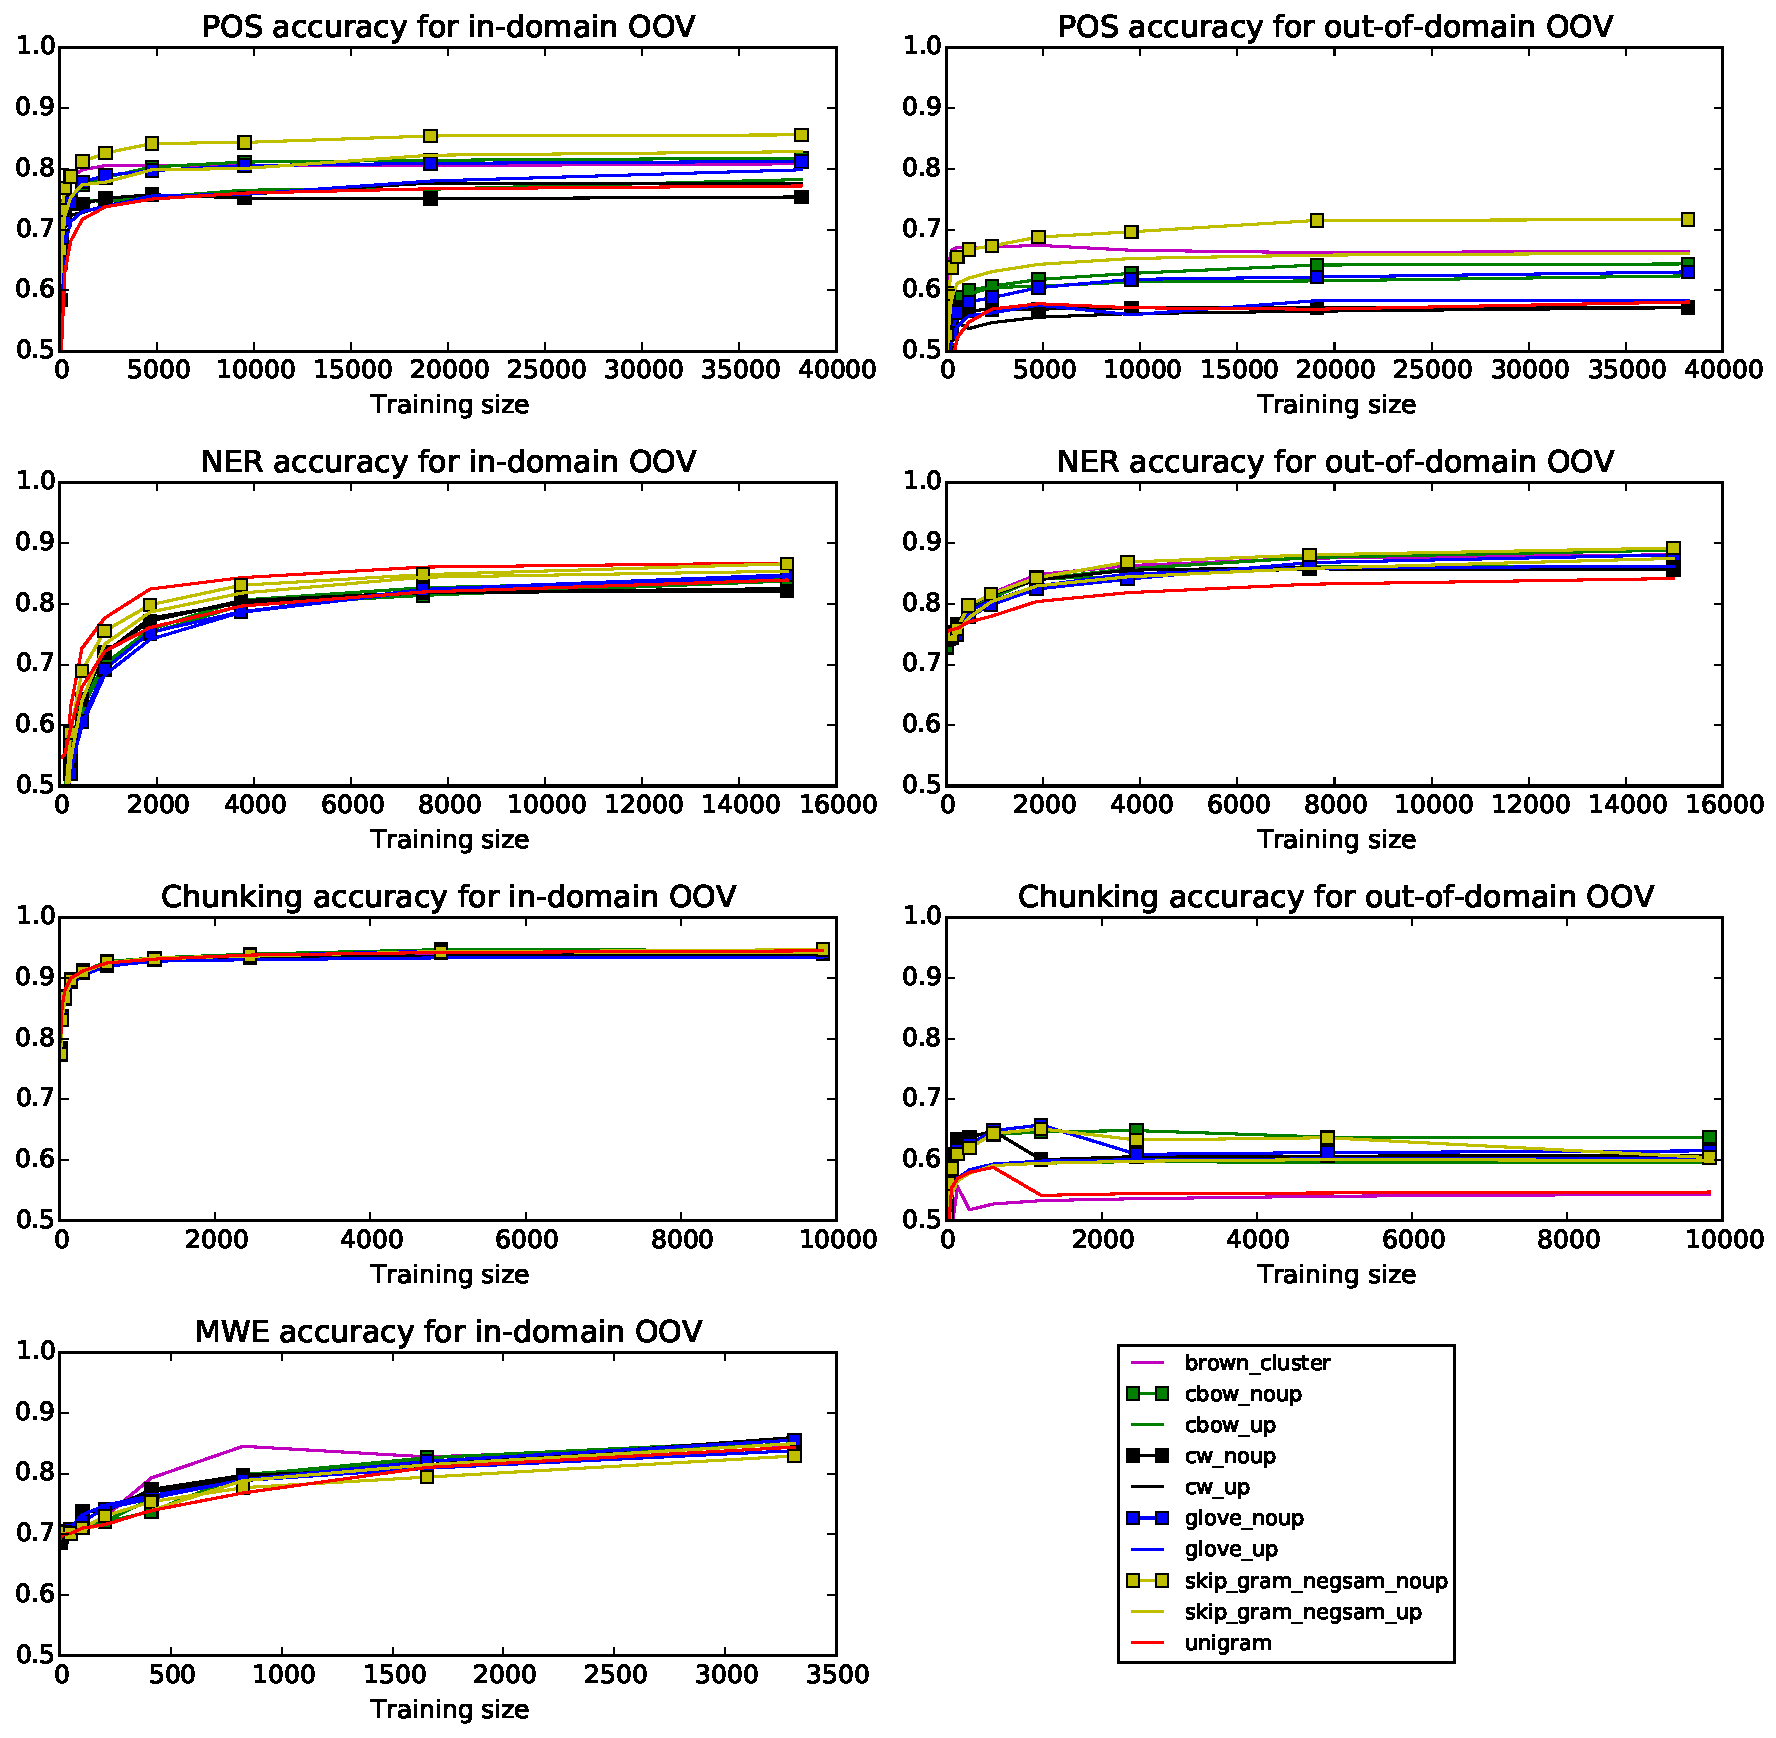
\includegraphics[scale=0.5]{plots/OOV-plots}
\caption{Out-of-vocabulary-words (OOV) accuracy for \textit{in-domain} and \textit{out-of-domain} test sets}
\label{OOV} 
\end{figure*}







%%% Local Variables: 
%%% mode: latex
%%% TeX-PDF-mode: t 
%%% TeX-master: "WordEmbEvaluation"
%%% End: 
